\subsubsection{5V Speisung}
\label{subsubsec:5V Speisung}

Der Mikrocontroller, sowie die Durchflussmessgeräte und das Display  werden mit 5V betrieben. Aus diesem Grund wurde eine 5V Speisung implementiert. Dazu wird der selbe Schaltspannungsregler wie bei der 12V Speisung in Kapitel \ref{subsubsec:12V Speisung} verwendet. Die Realisierung der 5V Speisung kann in Abbildung \ref{fig:Schema_Speisung_5V} betrachtet werden.\\

\paragraph{Schema}\mbox{}\\

Das Schema in Abbildung \ref{fig:Schema_Speisung_5V} kann wie bei der 12V Speisung gemäss Kapitel \ref{subsubsec:12V Speisung} in fünf Teile unterteilt werden. Da wären zuerst die Eingangskondensatoren, welche mit C31, C33 \& C35 realisiert sind. Diese Entstörstufe wird wiederum gefolgt von einem Spannungsteiler, welcher den Enable auf aktiv setzt. Der eigentliche Regler wird auch hier mittels des IC6, D5 \& L4 realisiert. Mittels zweier Spannungsteiler, wird die gewünschte Ausgangsspannung, sowie die \flqq Overvoltage-Protection\frqq~ eingestellt. Vor dem Ausgang der Schaltung ist dann erneut eine Kondensatorstufe implementiert, welche das Ausgangssignal glättet.

\begin{figure}[h!]
	\centering
	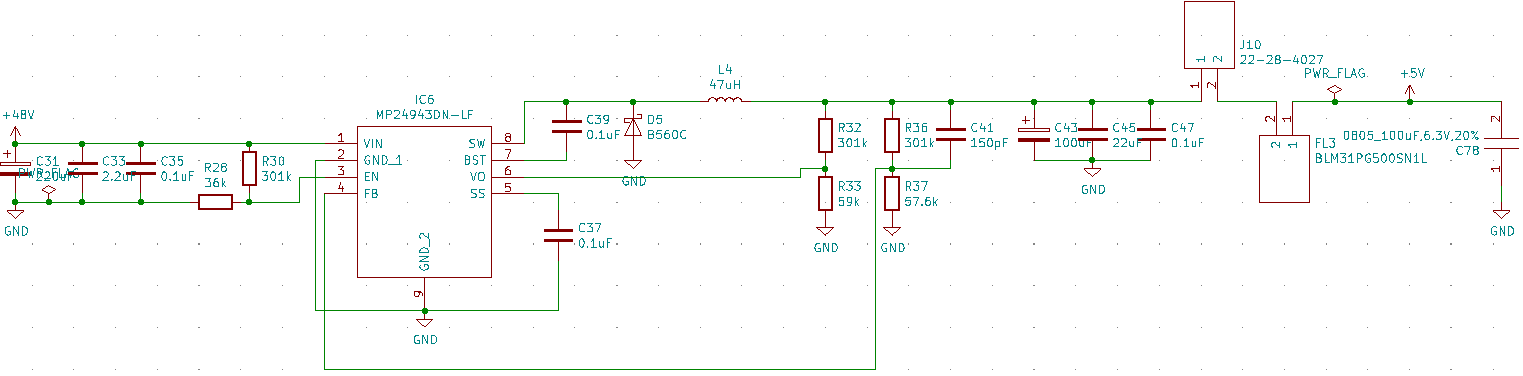
\includegraphics[width=\textwidth]{graphics/Schema_Speisung_5V.png}
	\caption{Schema der 5V Speisung}
	\label{fig:Schema_Speisung_5V}
\end{figure} 

\paragraph{Funktionsbeschrieb der Schaltung}\mbox{}\\

Auch bei der 5V Speisung wurde mittels R29 \& R31 ein Spannungsteiler realisiert, welcher das IC gemäss Kapitel \ref{subsubsec:12V Speisung} auf aktiv setzt.

Das Widerstandsverhältnis von R41 \& R42, welches die Ausgangsspannung definiert, wurde gemäss Formel \ref{equ:Ausgangsspannung_12V} berechnet. Somit ergeben sich für R41=301k$\Omega$ und für R42=57.6k$\Omega$, was einer Ausgangsspannung von 4.98V entspricht. \cite[S.10]{monolithic_power_systems_mp24943_2011} 

Beim Überspannungsschutz musste darauf geachtet werden, dass der Mikrokontroller AtMega2560-16AU nur in einem Spannungsbereich von 4.5V-5.5V betrieben werden darf. Die maximal verträgliche Eingangsspannung liegt laut Datenblatt bei 6V. Somit muss der Überspannungsschutz so gestaltet werden, dass die Schwelle von 6V nicht überschritten werden kann. Um dies erreichen zu können, wurde für R36=301k$\Omega$ und R37=53k$\Omega$ gewählt. Gemäss Formel \ref{equ:Vovp_12V} erhält man so eine Überspannungsschutzschwelle von 6V. \cite[S.1]{atmel_atmel_2014} \cite[S.10]{monolithic_power_systems_mp24943_2011}

Der interne Oszillator läuft wiederum bei einer Frequenz von 100kHz. Bei der ausgewählten Spule L4 von 47$\mu$H erhält man mittels Formel \ref{equ:12V_Spulenberechnung} ein $\Delta$I$_{L}$ von 0.953A. Auch hier gilt gemäss Datenblatt, dass die gewählte Spule auf mindestens 125\% des maximalen Ausgangsstroms von 3A ausgelegt werden soll. Auch der Gleichstromwiederstand der Spule sollte $ \leq \ $ 200m$\Omega$  sein. \cite[S.3]{monolithic_power_systems_mp24943_2011} \cite[S.10]{monolithic_power_systems_mp24943_2011} 

Mit den Kondensatoren C46, C48 \& C50 wird die Ausgangsspannung zum Abschluss auch noch geglättet. Bei den Eingangskondensatoren, sowie den Ausgangskondensatoren sollte es sich um low ESR Typen handeln. Auch hier wurde noch zum Abschluss ein Ferrit implementiert, welcher allfällige hochfrequente Störungen herausfiltern soll.

Auch bei der 5V Speisung wurde ein Jumper zu Testzwecken und zwei LED's implementiert. Ausserdem findet sich auch hier wieder ein Ferrit FL3, welcher letzte Störungen beseitigen soll. 


